
%%%%%%%%%%%%%%%%%%%%%%% file typeinst.tex %%%%%%%%%%%%%%%%%%%%%%%%%
%
% This is the LaTeX source for the instructions to authors using
% the LaTeX document class 'llncs.cls' for contributions to
% the Lecture Notes in Computer Sciences series.
% http://www.springer.com/lncs       Springer Heidelberg 2006/05/04
%
% It may be used as a template for your own input - copy it
% to a new file with a new name and use it as the basis
% for your article.
%
% NB: the document class 'llncs' has its own and detailed documentation, see
% ftp://ftp.springer.de/data/pubftp/pub/tex/latex/llncs/latex2e/llncsdoc.pdf
%
%%%%%%%%%%%%%%%%%%%%%%%%%%%%%%%%%%%%%%%%%%%%%%%%%%%%%%%%%%%%%%%%%%%


\documentclass[runningheads]{llncs}

\usepackage{amssymb}
\setcounter{tocdepth}{3}
\usepackage{graphicx}
\usepackage{hyperref}
\usepackage{url}
\urldef{\mailsa}\path|{aysengupta, xianlin, ksanjeev, sravichandra}@cs.stonybrook.edu|
\newcommand{\keywords}[1]{\par\addvspace\baselineskip
\noindent\keywordname\enspace\ignorespaces#1}
\newcommand{\swallow}[1]{ }

\begin{document}

\mainmatter  % start of an individual contribution

% first the title is needed
\title{Status Report: Team 8\\
Predicting Prices of Oil and Gold}

% a short form should be given in case it is too long for the running head
\titlerunning{Predicting the Prices of Oil and Gold}

% the name(s) of the author(s) follow(s) next
%
% NB: Chinese authors should write their first names(s) in front of
% their surnames. This ensures that the names appear correctly in
% the running heads and the author index.
%
\author{Ayush Sengupta \and Benjamin Lin \and Komal Sanjeev \and Sreevathsan Ravichandran}
%
\authorrunning{Ayush Sengupta \and Benjamin Lin \and Komal Sanjeev \and Sreevathsan Ravichandran}
% (feature abused for this document to repeat the title also on left hand pages)

% the affiliations are given next; don't give your e-mail address
% unless you accept that it will be published
\institute{Department of Computer Science, Stony Brook University,\\
Stony Brook, NY 11794-4400\\
\mailsa\\
\url{http://www.cs.stonybrook.edu/~skiena/591/projects}}

%
% NB: a more complex sample for affiliations and the mapping to the
% corresponding authors can be found in the file "llncs.dem"
% (search for the string "\mainmatter" where a contribution starts).
% "llncs.dem" accompanies the document class "llncs.cls".
%

\toctitle{Lecture Notes in Computer Science}
\tocauthor{Authors' Instructions}
\maketitle

\swallow{   % DO NOT BOTHER WITH THIS
\begin{abstract}
The abstract should summarize the contents of the paper and should
contain at least 70 and at most 150 words. It should be written using the
\emph{abstract} environment.
\keywords{We would like to encourage you to list your keywords within
the abstract section}
\end{abstract}
}

\section{Background Updates}
 
\subsection{Objective}
Our objective is to predict the prices of Oil and Gold on January 1st 2015 as of December 1st in 2014 (a month in advance).

\subsection{Baseline Models}
In order to illustrate an improvement in the accuracy of our prediction, we compare our current autoregressive and multiple linear regressive models to the following baseline models:

\begin {itemize}
\item \textbf{Oil/Gold price is the same as the previous day's price:} \\
$P_{t}$ = $P_{t-1}$\\
\item \textbf{Oil/Gold price is a weighted mean of price of previous 3 days:} \\
$P_{t}$ = $\frac{1}{\{k(k+1)\}^2}\sum\limits_{i=1}^k (k-i+1)^3P_{t-i}$
\end {itemize}

\subsubsection {Error Metrics for Baseline Models} The following are the error metrics for our baseline models: \\

\begin{tabular}{|l|l|l|l|}
\hline
Model & Relative Error & Mean Absolute Error & RMSE \\ \hline
$ Model 0.0 $ & $6.73746$ & $5.384215$ & $7.101763$ \\ \hline
$ Model 0.1 Average $ & $7.27174$ & $5.761054$ & $7.754635$\\ \hline
\end{tabular}

[ADD: PLOT]

\subsection{Autoregressive and Multiple Linear Regressive Models?}

\subsection{Spot price prediction using Futures prices}
[Futures???]\\


\newpage
\section{Data Matrices}
Our data consists of multiple time series of monthly Oil and Gold prices, and the following macroeconomic factors:

\begin {itemize}
\item S\&P 500 Index
\item New York Stock Exchange Index (NYSE)
\item US Dollar Index
\item Consumer Sentiment Index (CSI)
\item EURO-USD Conversion Rate
\end {itemize}
 
\begin{figure}
\centering
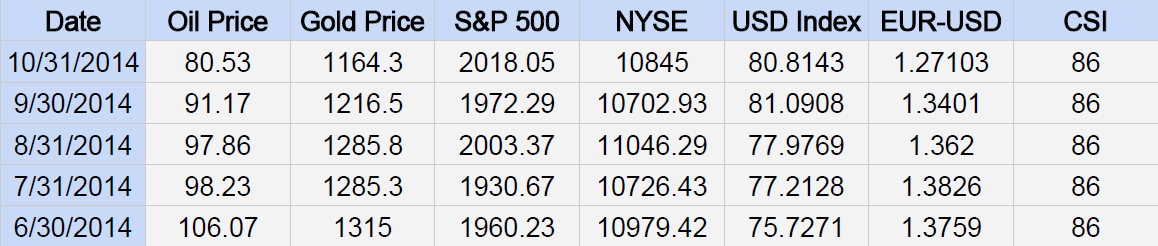
\includegraphics[width=\textwidth]{DataMatrices.png}
\caption{Data frame for oil and gold price and its related economic factors}
\label{fig:DataMatrices.png}
\end{figure}

\begin{figure}
\centering
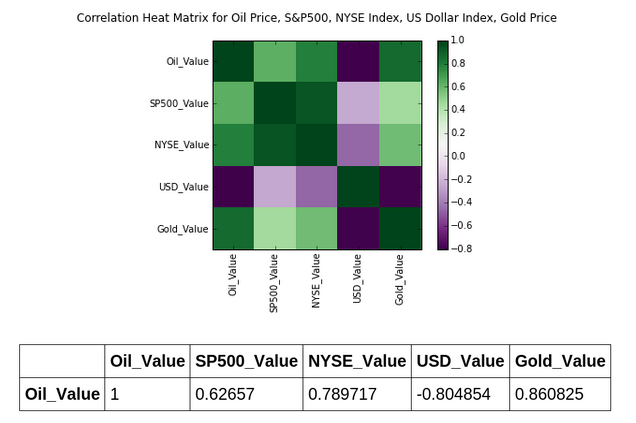
\includegraphics[width=\textwidth]{HeatMap_Oil_Daily.png}
\caption{Correlation Heat Map for Oil Price and related macroeconomic factors}
\label{fig:HeatMap_Oil.png}
\end{figure}

\begin{center}
\begin{tabular}{|c|c|c|c|c|c|}
\hline
\multicolumn{6}{|c|}{Correlation Matrix} \\
\hline
$ $ & $Oil Price$ & $ S\&P 500 $ & $ NYSE $ & $ USD Index $ & $Gold Price$ \\ [0.5ex]  \hline
$Oil Price$ & $ 1 $ & $0.718178$ & $0.805763$ & $-0.77365$ & $0.872$ \\ \hline
\end{tabular}
\end{center}

The correlation heat map in \autoref{fig:HeatMap_Oil.png}, and the corresponding table containing correlation coefficients show the correlation between the price of oil and related economic factors. They indicate a high correlation between oil price and certain macroeconomic factors - S\&P 500, NYSE, US Dollar Index, Gold Price.

\begin{figure}
\centering
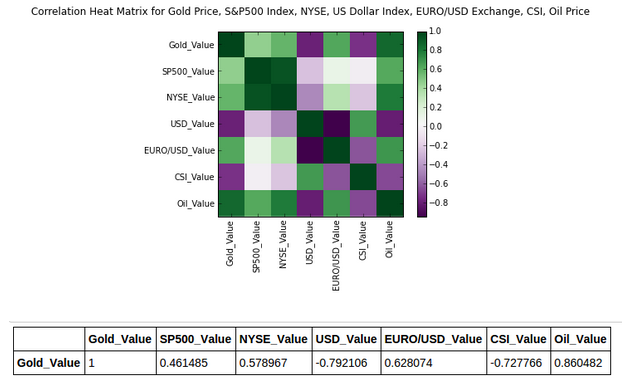
\includegraphics[width=\textwidth]{HeatMap_Gold_Daily.png}
\caption{Heat Map and Correlation Coefficient Matrix for Gold price and its related macroeconomic factors}
\label{fig:HeatMap_Gold_Daily.png}
\end{figure}

\begin{center}
\begin{tabular}{|c|c|c|c|c|c|c|c|}
\hline
\multicolumn{8}{|c|}{Correlation Matrix} \\
\hline
$ $ & $Gold Price$ & $ S\&P 500 $ & $ NYSE $ & $ USD $ & $EUR-USD$ & $CSI$ &$Oil Price$ \\ [0.5ex]  \hline
$Gold Price$ & $ 1 $ & $0.461485$ & $0.578967$ & $-0.792106$ & $0.628074$ & $-0.727766$ & $0.860482$ \\ \hline
\end{tabular}
\end{center}

The correlation heat map in \autoref{fig:HeatMap_Gold_Daily.png}, and the corresponding table containing correlation coefficients show the correlation between the price of oil and related economic factors. They indicate a high correlation between Gold Price and certain macroeconomic factors - US Dollar Index, EURO-USD Conversion Rate and Oil Price.


\subsection{Data Sources}
\noindent For both the daily and monthly data, they are obtained from \\
Oil Price: \url{https://www.quandl.com} \\ 
Gold Price: \url{https://www.quandl.com} \\
SP500: \url{https://www.quandl.com} \\
NYSE: \url{https://www.quandl.com} \\
USD: \url{https://www.quandl.com} \\
EURO/USD: \url{https://www.quandl.com} \\
CSI: \url{http://future.aae.wisc.edu/data/monthly_values/by_area/998?grid=true} \\

[ADD: HOW SATISFIED ARE YOU WITH THE DATA YOU COLLECTED?]

\newpage
\section{Development/Evaluation Environment}

\begin{figure}
\centering
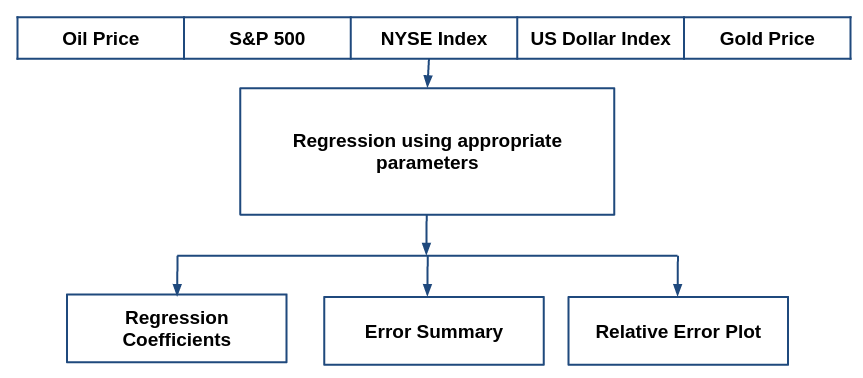
\includegraphics[width=\textwidth]{DevelopmentFlowchart.png}
\caption{The development and evaluation environment for the oil price prediction with economic factors involved}
\label{fig:DevelopmentFlowchart.png}
\end{figure}

\noindent \autoref{fig:DevelopmentFlowchart.png} shows the work flow of our prediction model. The model uses past prices of oil/gold, combined with certain macroeconomic factors, and performs regression to make predictions. The accuracy of the model is then determined on the basis of error metrics. \\

\noindent A data frame containing multiple time series of oil/gold prices and related macroeconomic factors is generated. A parameter corresponding to each of these factors is also passed as a part of the input to the model. This parameter is a number which represents the number of values of the past days of that factor which will be regressed by the model. We can also choose not to consider a particular factor by assigning $0$ to the parameter.\\

\noindent The model is trained on the initial 60\% of the time series, and tested on the remaining 40\%. The model tries generate a linear function while assigning coefficients for each of these economic factors. These regression coefficients are then used to make predictions for the next month. \\  

\noindent \textbf	{Error Summary.} The following error metrics are calculated - Mean Relative Error, Mean Absolute Error, and Root Mean Square Error. A histogram of the relative error frequencies is also generated. \\

[ ADD ]

%\noindent We synthesize the economic factors for predicing the oil price into a data frame, then we write a function to generate a multiple linear regression model with auto regressive feature [CHECK: is "multiple linear regression model with auto regressive feature" a good alternative wording or shall we continue use "auto regressive model taking economic factors", omitting "linear regression"?]. Then we write a function to run linear regression using appropriate parameters. After executing the function, we obtain the regression coefficients. Based on that, we can continue derive error summaries and make relative error plots. \\

\newpage

\section{Current Model and Baseline}

We have developed autoregressive and multiple linear regressive models to make oil and gold price predictions.

[ ADD ]

\subsubsection{Autoregressive Model}
Autoregressive models are based purely on historical prices. They model the time series as a linear function of the values of the past 'p' days.\\

$ X_{t} = c + \sum\limits_{i=1}^p \varphi_{t-i}X_{t-i} + \epsilon_{t}$. \\

\noindent The Odinary Least Squares (OLS) method is used to estimate the parameters in the regression model. It tries to minimize the sum of squares of vertical distances between the predicted and the actual values. 

\subsubsection{Autoregressive and Multiple Linear Regressive Model}
Linear regression models the relationship of two variables - a dependent variable and an explanatory variable using a linear function. The process of modeling a variable based on more than one explanatory variables is called Multiple Linear Regression. \\
   
\noindent An initial model is developed which is a purely autoregressive function. Then, the model is expanded to incorporate the factors which are highly correlated to the price of oil/gold we are trying to predict. As each factor is incorporated into the model, we perform a comparison of the error metrics between these models and try to estimate the model which makes predictions which best accuracy.\\

For predicting the price of oil, the following macroeconomic factors are taken into consideration:
\begin {itemize}
\item S\&P 500 Index
\item NYSE Index
\item US Dollar Index
\item Gold Price
\end {itemize}

For predicting the price of gold, the following factors macroeconomic are taken into consideration:
\begin {itemize}
\item S\&P 500 Index
\item NYSE Index
\item US Dollar Index
\item EURO-USD Exchange Rate
\item Consumer Sentiment Index
\item Oil Price
\end {itemize}


\subsubsection{Autoregressive Moving Average Model (ARMA)}
ARMA models are used to understand and predict time series values as a function of two polynomials, an autoregressive function, and a moving average function. 
\\

$ X_{t} = c + \sum\limits_{i=1}^p \varphi_{t-i}X_{t-i} + \epsilon_{t} + \sum\limits_{i=1}^q \theta_{t-i}X_{t-i}$.\\

In ARMA (p,q), p is referred to as the order of the autoregressive part and q is referred to as the order of the moving average part, i.e, the model is described using p autoregressive terms and q moving average terms.\\ 

[ ADD ]

\subsubsection {Why other autoregressive models fail to perform much better than baseline?}
ACF: Autocorrelation Factor
PACF: Partial autocorrelation Factor(auto-correlation with the linear dependence between variables removed)
\\

[ ADD ]

\subsection {OIL}

\subsubsection {Performance of Autoregressive Models against Baseline Models} A comparison.\\

[ CHANGE ]

\begin{figure}
\centering
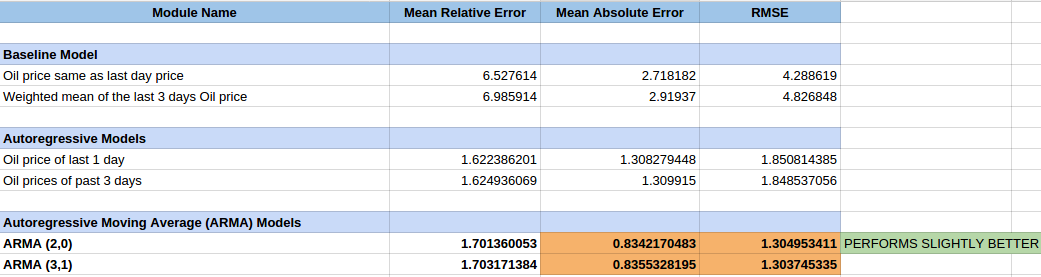
\includegraphics[width=\textwidth]{OILAutoAgainstBase_Daily.png}
\caption{Current Autoregressive Models against base}
\label{fig:OILAutoAgainstBase_Daily.png}
\end{figure}

\begin{figure}
\centering
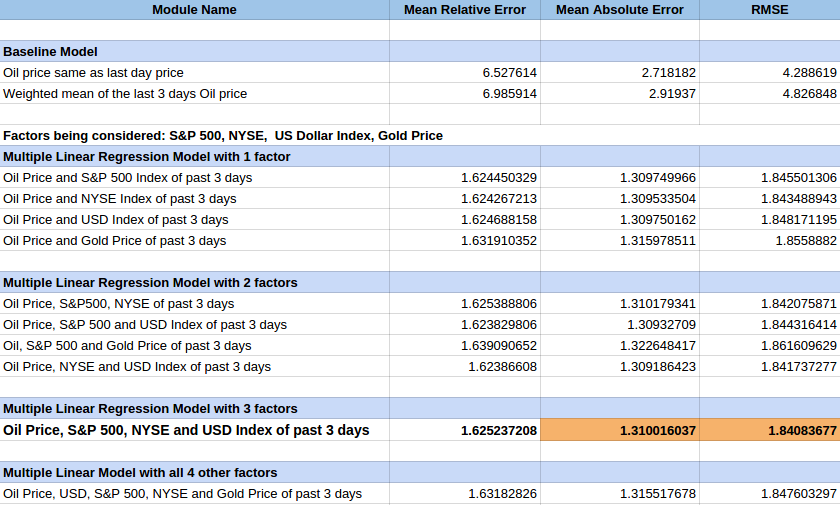
\includegraphics[width=\textwidth]{OILMLRAgainstBase_Daily.png}
\caption{Current Multiple Linear Regression Models against base}
\label{fig:OILMLRAgainstBase_Daily.png}
\end{figure}


\noindent\textbf{Comparison Summary} \\
Autoregressive Models "ARMA(2,0)" and "ARMA(3,1)" have lower errors than the baseline models. ARMA(2,0) has slightly lower Mean Relative Error and Mean Absolute Error than ARMA(3,1), but a slightly higher RMSE than ARMA(3,1). \\
Multiple Linear Regression Model "Oil Price, S\&P 500, NYSE and USD Index of past 3 days" has the lowest RMSE. 
It has lower errors than the baseline models. \\

[ EDIT ]


\subsection {GOLD}

\subsubsection {Performance of Autoregressive Models against Baseline Models} A comparison.\\

\noindent\textbf{Current Multiple Linear Regression Models}
Note: After generating the correlation coefficient heat map [Fig 4.], we only concerning the combination of Gold Price, USD, EURO/USD, CSI, Oil Price for predicting gold price. \\

\noindent\textbf{Performance against Baseline Models}

[ CHANGE]

\begin{figure}
\centering
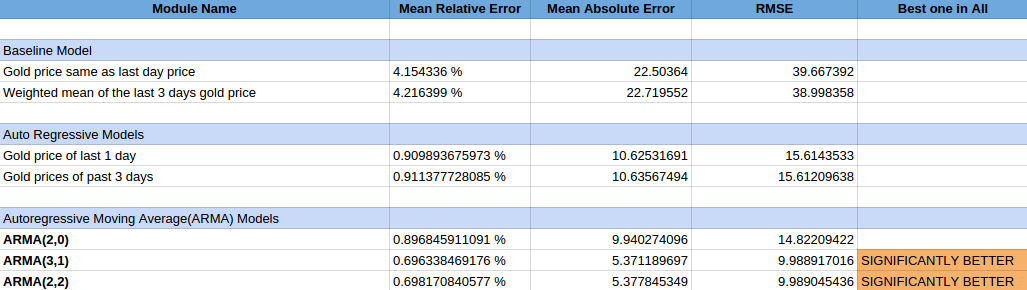
\includegraphics[width=\textwidth]{GoldAutoAgainstBase_Daily.png}
\caption{Current Autoregressive Models against base}
\label{fig:GoldAutoAgainstBase_Daily.png}
\end{figure}

\begin{figure}
\centering
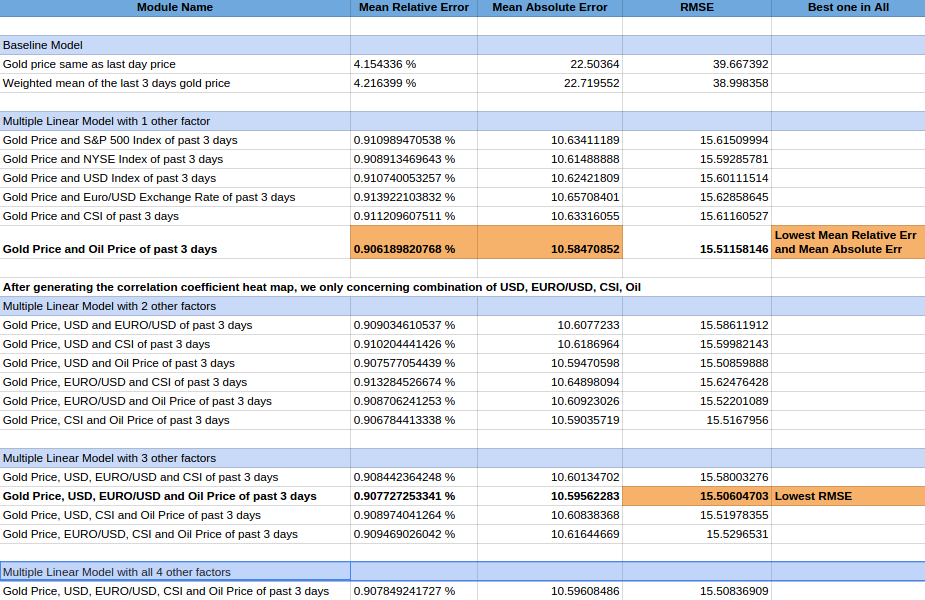
\includegraphics[width=\textwidth]{GoldMLRAgainstBase_Daily.png}
\caption{Current Autoregressive Models against base}
\label{fig:GoldMLRAgainstBase_Daily.png}
\end{figure}

[ EDIT ]

\noindent\textbf{Comparison Summary} \\
Autoregressive Models "ARMA(3,1)" and "ARMA(2,2)" have significantly lower errors than the baseline models. ARMA(3,1) has slightly lower errors 
than ARMA(2,2). \\
Multiple Linear Regression Model "Gold Price and Oil Price of past 3 days" has the lowest mean relative error and the lowest mean absolute error; 
 "Gold Price, USD, EURO/USD and Oil Price of past 3 days" has the lowest RMSE.
Both have significant lower errors than the baseline models. \\

\subsection{Summary}

\newpage

\section{Current Prediction and Next Steps}

\subsection {Current Prediction}
\noindent The predicted price of WTI Crude Oil on Dec 1 as of Nov 1 is \\
\textbf{00.00 USD per Barrel} \\

\noindent The predicted price of Gold on Dec 1 as of Nov 1 \\
\textbf{0000.00 USD per ounce} \\

\subsection {Next Steps}

S\&P 1200 Global: \url {http://en.wikipedia.org/wiki/S%26P_Global_1200} \\

\noindent We will further investigate how we may include futures price as one of the economic factors to help predict oil and gold price. \\

\noindent [ADD "Present what you will do next to get a complete predictive model.  Discuss any difficulties you will have to overcome in building a good model"]

\subsubsection*{Acknowledgments.} Here acknowledge any other people who helped with this project.

\section{Bibliography}\label{references}

The correct BibTeX entries for the Lecture Notes in Computer Science
volumes can be found at the following Website shortly after the
publication of the book:
\url{http://www.informatik.uni-trier.de/~ley/db/journals/lncs.html}

For citations in the text please use
square brackets and consecutive numbers: \cite{jour}, \cite{lncschap},
\cite{proceeding1} -- provided automatically
by \LaTeX 's \verb|\cite| \dots\verb|\bibitem| mechanism.

Please base your references on the
examples below. 
The following section shows a sample reference list with entries for
journal articles \cite{jour}, an LNCS chapter \cite{lncschap}, a book
\cite{book}, proceedings without editors \cite{proceeding1} and
\cite{proceeding2}, as well as a URL \cite{url}.
Please note that proceedings published in LNCS are not cited with their
full titles, but with their acronyms!

\begin{thebibliography}{4}

\bibitem{jour} Smith, T.F., Waterman, M.S.: Identification of Common Molecular
Subsequences. J. Mol. Biol. 147, 195--197 (1981)

\bibitem{lncschap} May, P., Ehrlich, H.C., Steinke, T.: ZIB Structure Prediction Pipeline:
Composing a Complex Biological Workflow through Web Services. In: Nagel,
W.E., Walter, W.V., Lehner, W. (eds.) Euro-Par 2006. LNCS, vol. 4128,
pp. 1148--1158. Springer, Heidelberg (2006)

\bibitem{book} Foster, I., Kesselman, C.: The Grid: Blueprint for a New Computing
Infrastructure. Morgan Kaufmann, San Francisco (1999)

\bibitem{proceeding1} Czajkowski, K., Fitzgerald, S., Foster, I., Kesselman, C.: Grid
Information Services for Distributed Resource Sharing. In: 10th IEEE
International Symposium on High Performance Distributed Computing, pp.
181--184. IEEE Press, New York (2001)

\bibitem{proceeding2} Foster, I., Kesselman, C., Nick, J., Tuecke, S.: The Physiology of the
Grid: an Open Grid Services Architecture for Distributed Systems
Integration. Technical report, Global Grid Forum (2002)

\bibitem{url} National Center for Biotechnology Information, \url{http://www.ncbi.nlm.nih.gov}

\end{thebibliography}


\end{document}
